\documentclass{article}
\author{}

\usepackage{graphicx}
\usepackage{wrapfig}
\usepackage{enumerate}
\usepackage{hyperref}
\usepackage{float}
\usepackage[margin = 2.25cm]{geometry}
\usepackage[table]{xcolor}
\usepackage{fancyhdr}
\hypersetup{
  colorlinks = true,
  urlcolor = blue
}
\setlength\parindent{0pt}
\pagestyle{fancy}
\fancyhf{}
\rhead{College of Engineering, Construction and Living Sciences\\Bachelor of Information Technology}
\lfoot{Practical 17 React 2: Components \& Props \\Version 1, 2020}
\rfoot{\thepage}

\begin{document}

\begin{figure}
	\centering
	
\includegraphics[width=50mm]{./img/logo.png}
\end{figure}

\title{College of Engineering, Construction and Living Sciences\\Bachelor of Information Technology\\IN608: Intermediate Application Development Concepts\\Level 6, Credits 15\\\textbf{Practical 17 React 2: Components \& Props}} 
\date{}
\maketitle

\textbf{Due Date:} /09/2020 at 5pm \\

In this practical, you will complete a series of tasks covering today's lecture. This practical is worth 1\% of the final mark for the IN608: Intermediate Application Development Concepts course. \\

Before you start, in your practicals repository, create a new branch called \textbf{17-practical}.

\section*{Task} 
Create a React app called \texttt{practical17components}. \texttt{cd} to \texttt{practical17components} \& install the following package:
\begin{itemize}
  \item React router - \texttt{npm i react-router}
\end{itemize}

\subsection*{Expected Output} 
Run the command \texttt{npm start} then navigate to \href{http://localhost:3000/}{http://localhost:3000/} \\

\begin{figure}[H]
  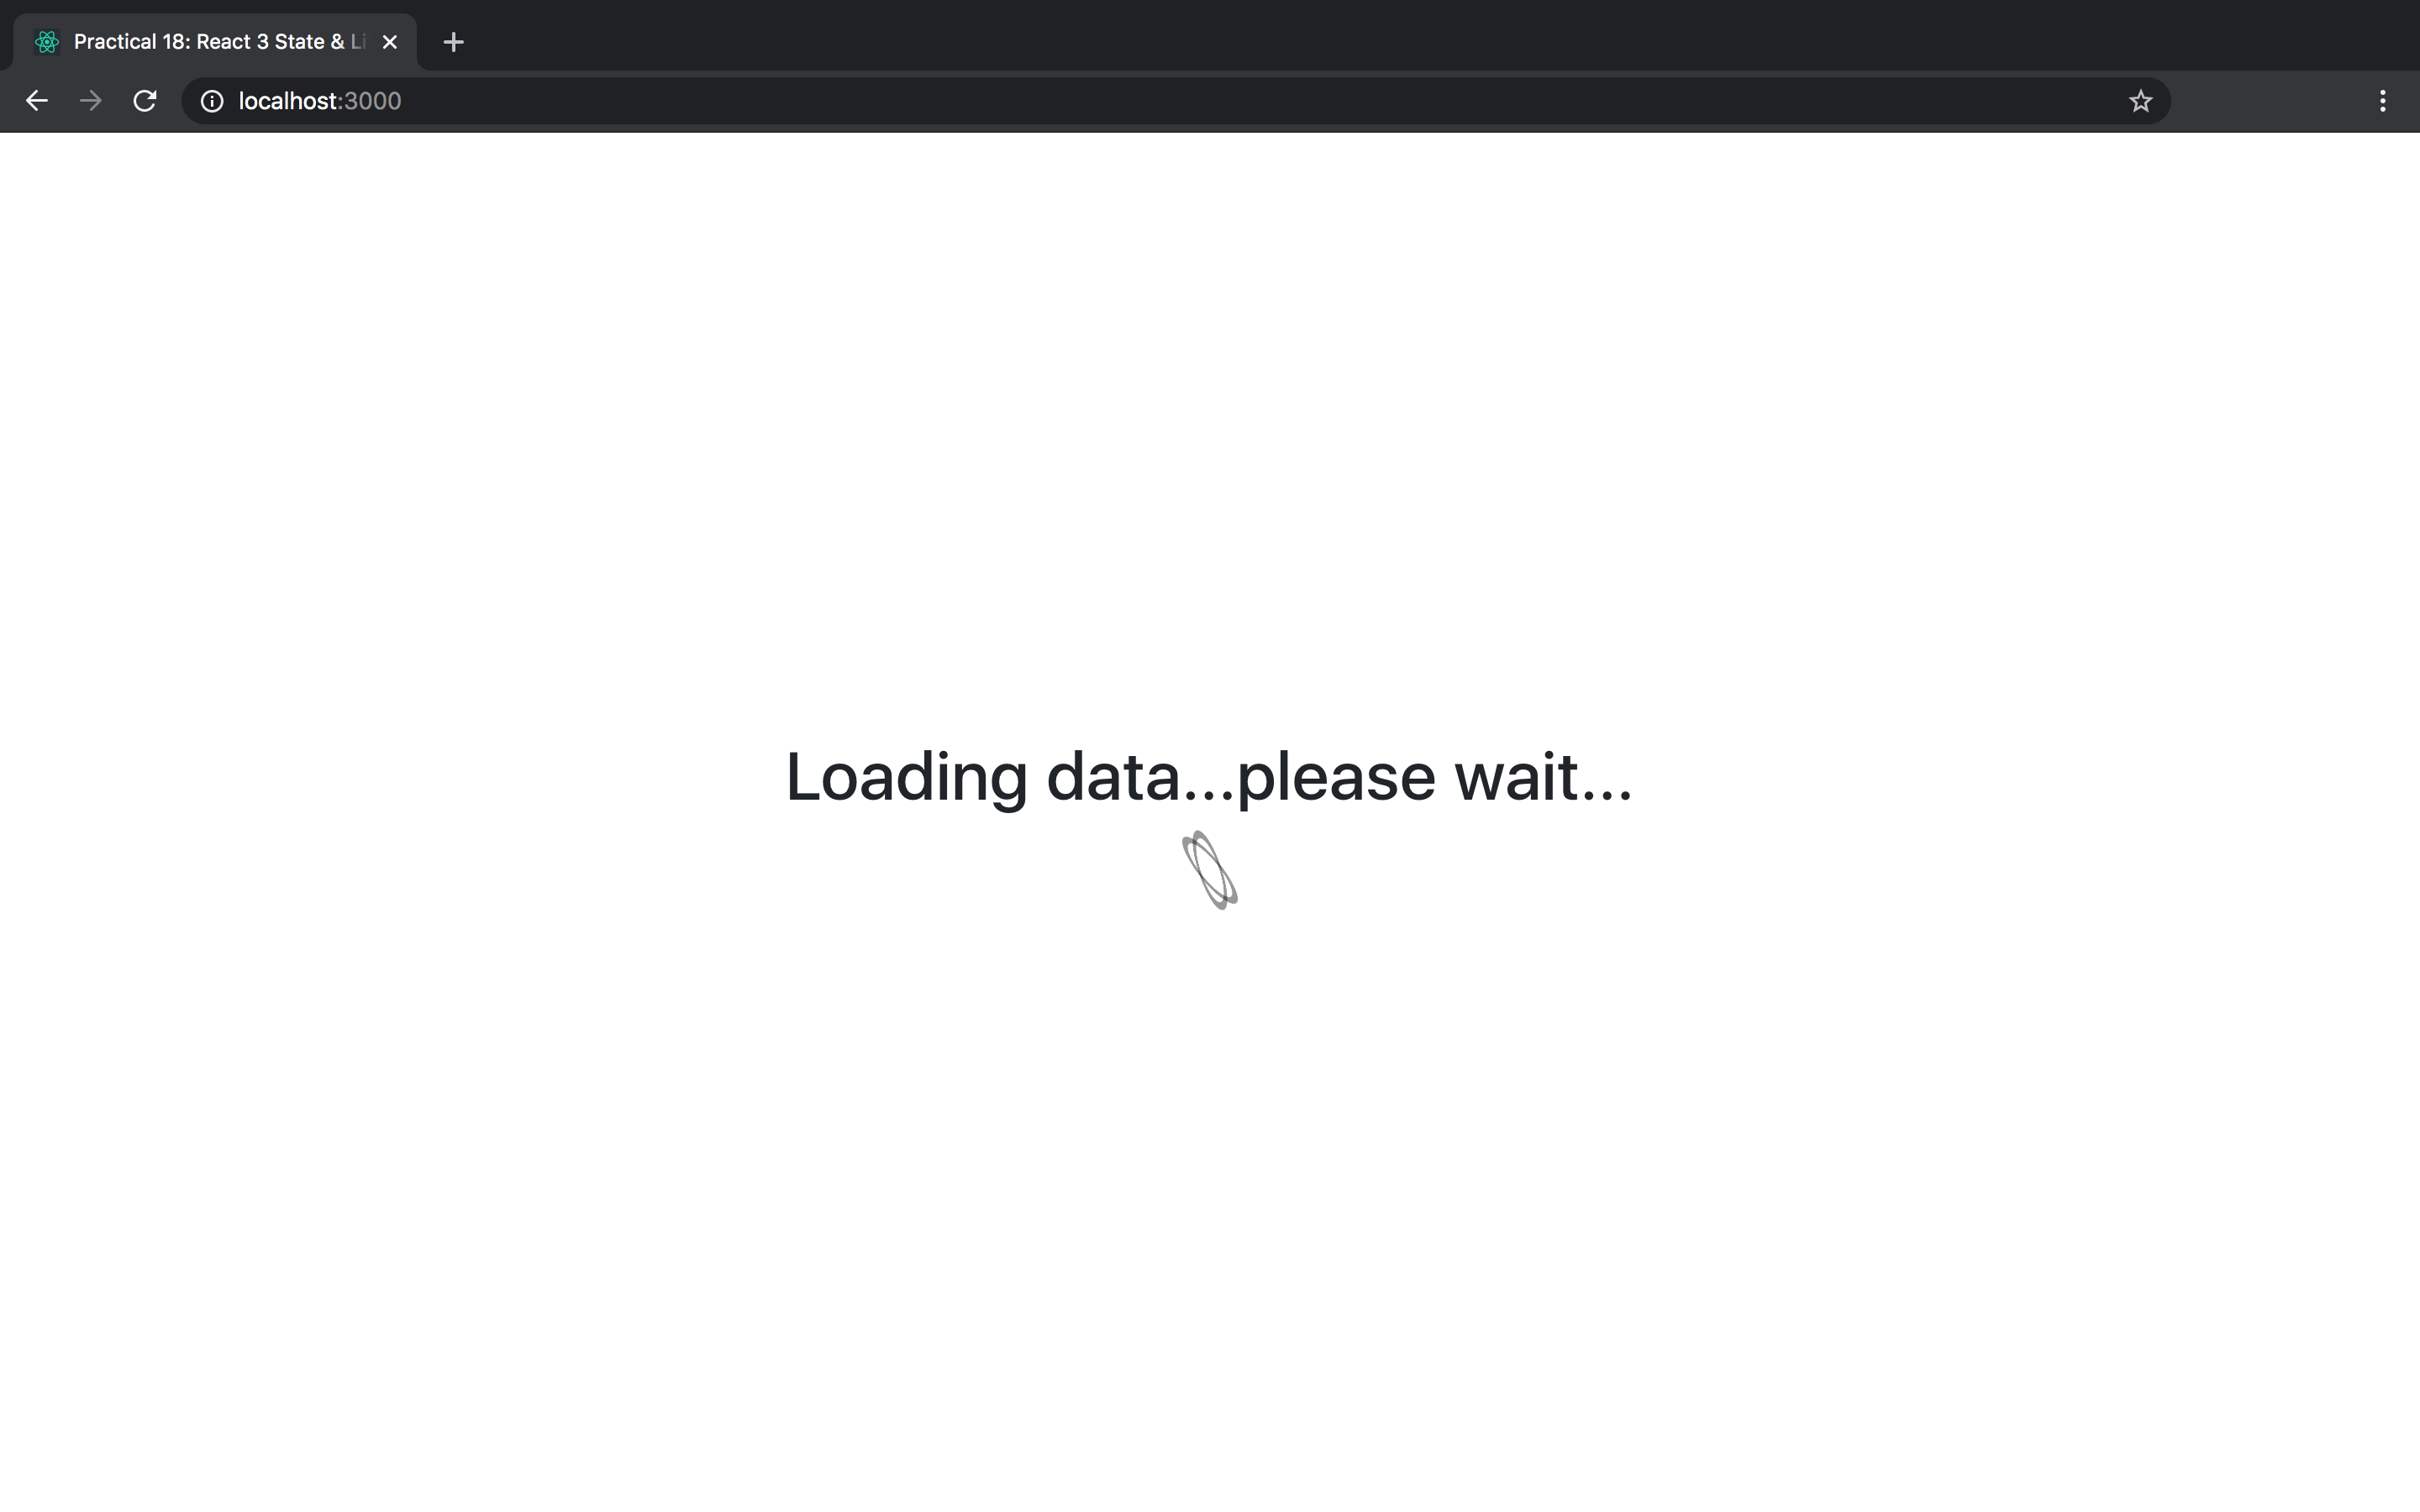
\includegraphics[width=175mm, height=105mm]{./img/18-expected-opentdb-1.png}
  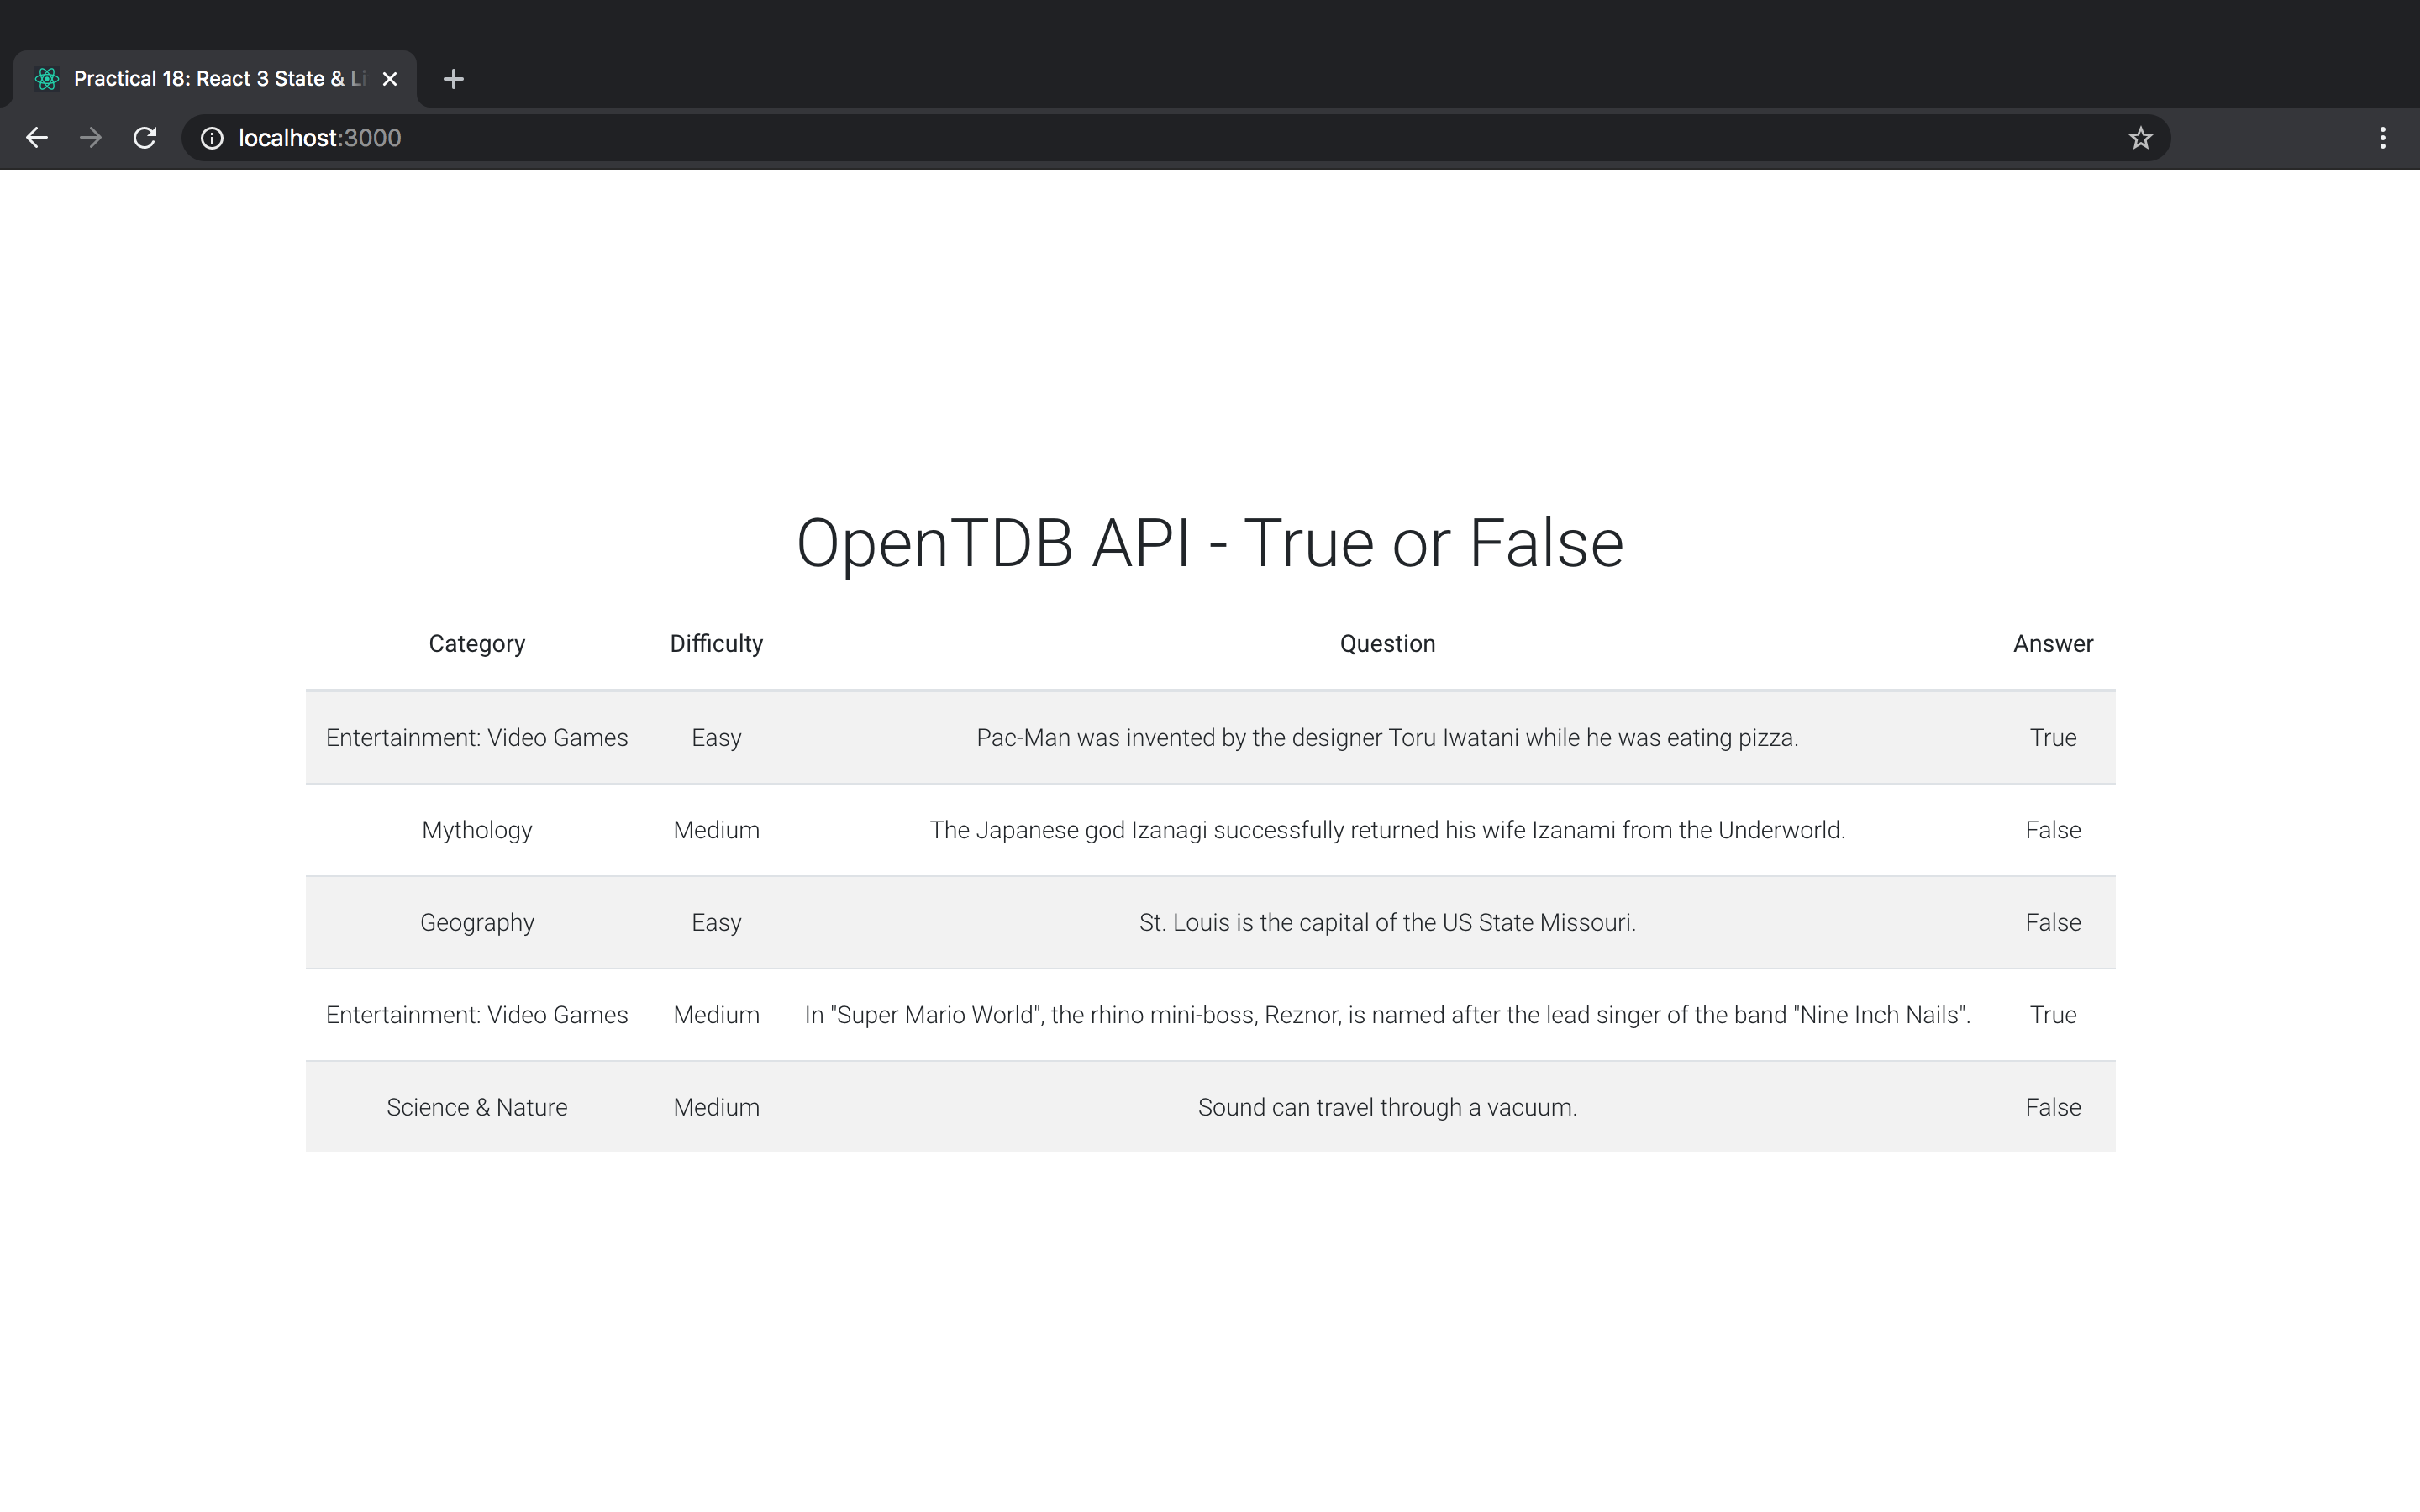
\includegraphics[width=175mm, height=105mm]{./img/18-expected-opentdb-2.png}
\end{figure}

\begin{figure}[H]
  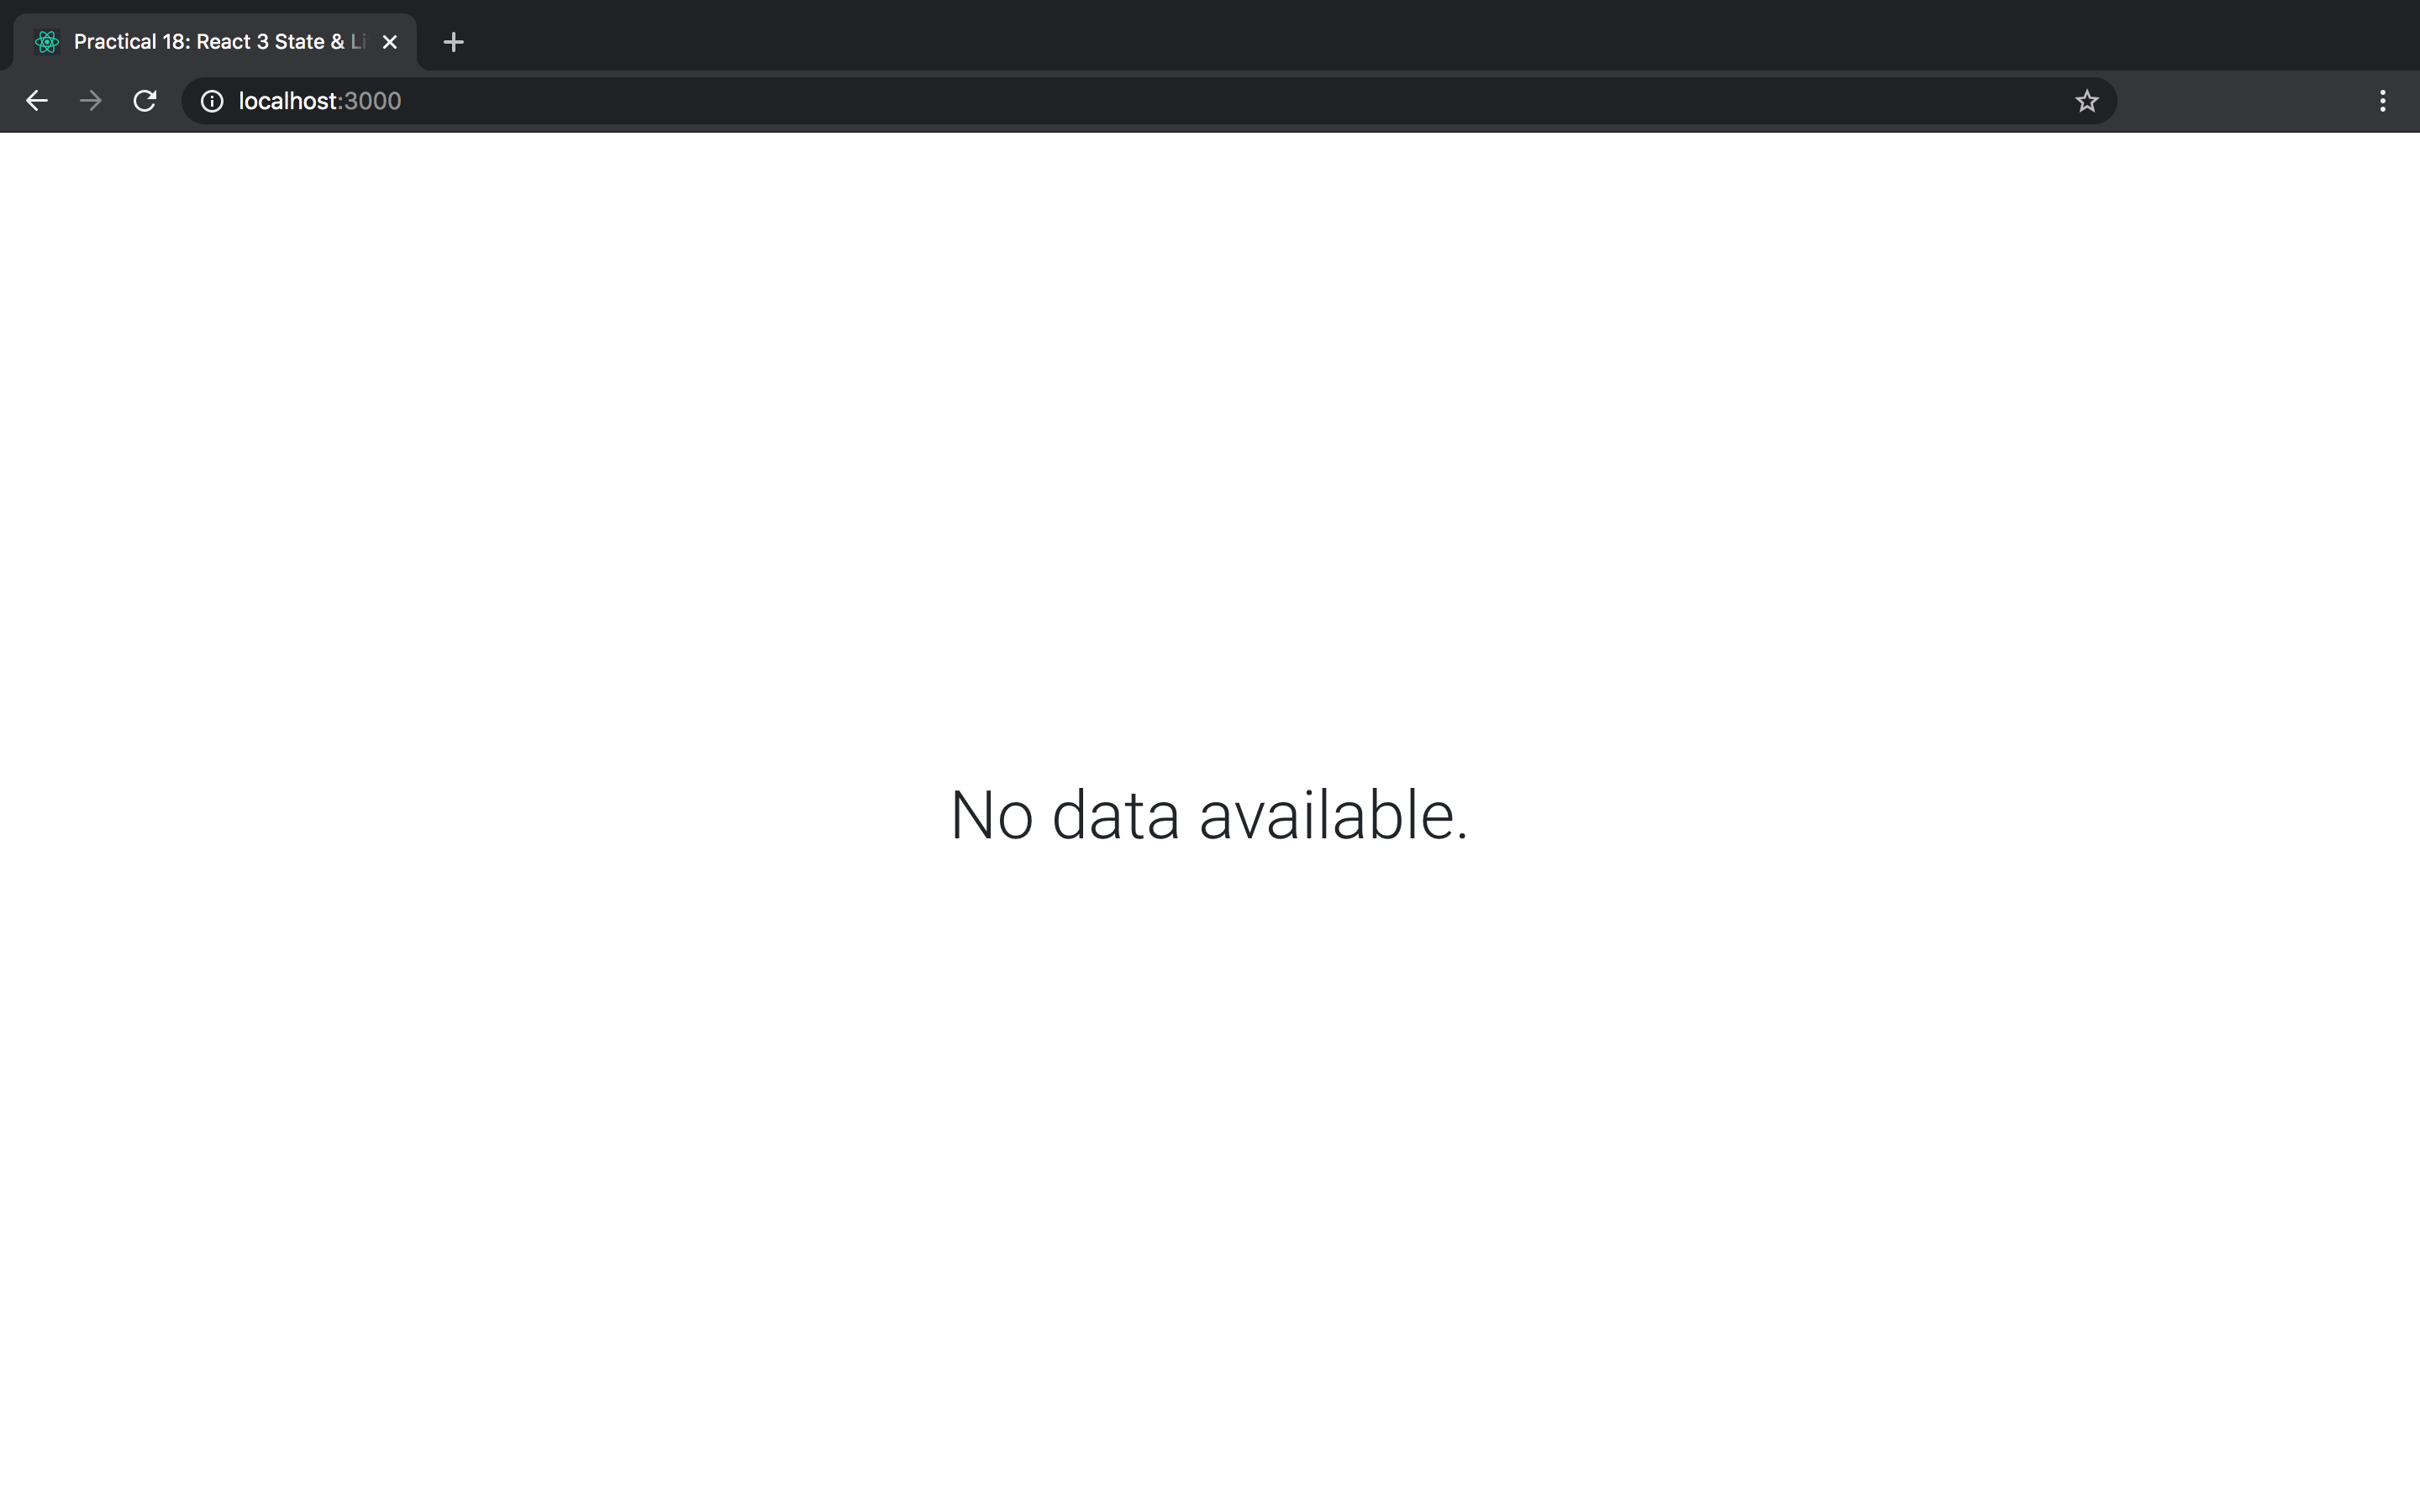
\includegraphics[width=175mm, height=105mm]{./img/18-expected-opentdb-3.png}
  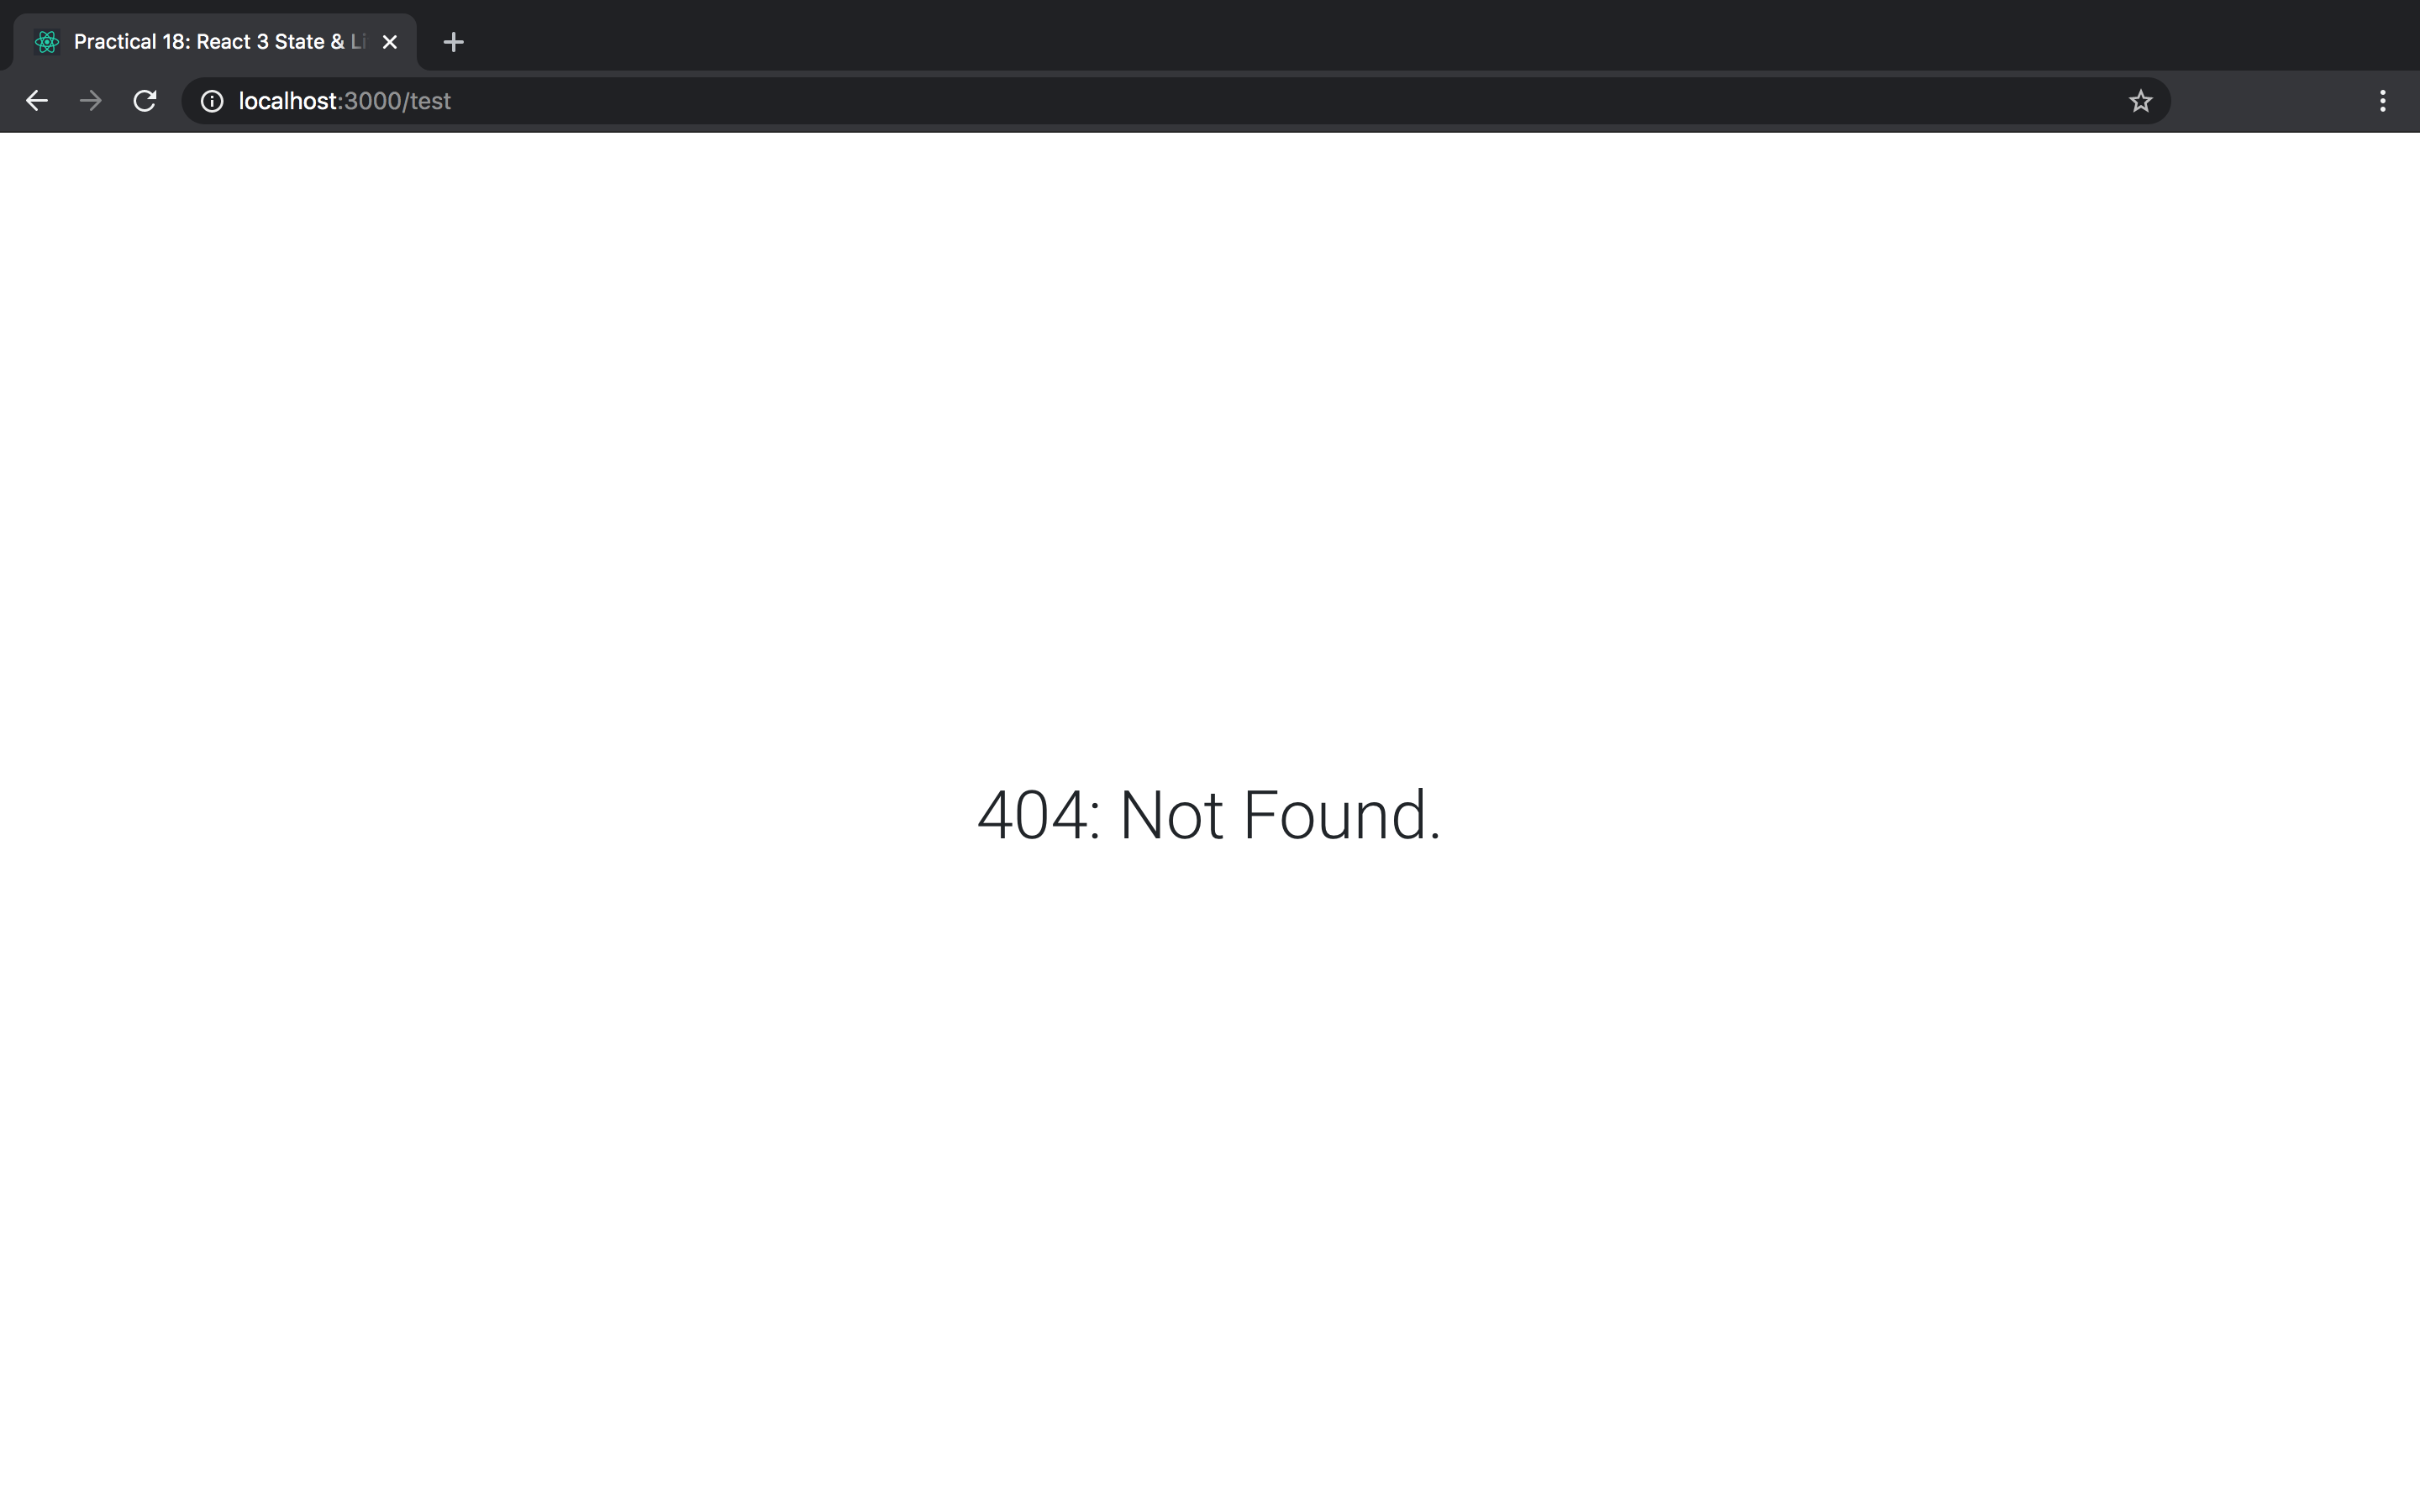
\includegraphics[width=175mm, height=105mm]{./img/18-expected-opentdb-4.png}
\end{figure}

\textbf{Deployment link:} \href{https://int-app-dev-practical-18.herokuapp.com/}{https://int-app-dev-practical-08.herokuapp.com/} 

\subsection*{Resources} 
\begin{itemize}
  \item \href{https://www.npmjs.com/package/react-router/}{React router}
\end{itemize}
 
\end{document}